% CVPR 2022 Paper Template
% based on the CVPR template provided by Ming-Ming Cheng (https://github.com/MCG-NKU/CVPR_Template)
% modified and extended by Stefan Roth (stefan.roth@NOSPAMtu-darmstadt.de)

\documentclass[10pt,twocolumn,letterpaper]{article}

%%%%%%%%% PAPER TYPE  - PLEASE UPDATE FOR FINAL VERSION
% \usepackage[review]{cvpr}      % To produce the REVIEW version
% \usepackage{cvpr}              % To produce the CAMERA-READY version
\usepackage[pagenumbers]{cvpr} % To force page numbers, e.g. for an arXiv version

% Include other packages here, before hyperref.
\usepackage{graphicx}
\usepackage{amsmath}
\usepackage{amssymb}
\usepackage{booktabs}
\usepackage{multicol}
\usepackage{multirow}
\usepackage{makecell}
\usepackage{algorithm}
\usepackage{algpseudocode}
\usepackage[table]{xcolor}
\usepackage{comment}
\usepackage{tabularx}

% \usepackage[accsupp]{axessibility}  % Improves PDF readability for those with disabilities.

\def\mathbi#1{\textbf{\em #1}}
\DeclareMathOperator*{\argmax}{arg\,max}
\DeclareMathOperator*{\argmin}{arg\,min}

% It is strongly recommended to use hyperref, especially for the review version.
% hyperref with option pagebackref eases the reviewers' job.
% Please disable hyperref *only* if you encounter grave issues, e.g. with the
% file validation for the camera-ready version.
%
% If you comment hyperref and then uncomment it, you should delete
% ReviewTempalte.aux before re-running LaTeX.
% (Or just hit 'q' on the first LaTeX run, let it finish, and you
%  should be clear).
\usepackage[pagebackref,breaklinks,colorlinks]{hyperref}


% Support for easy cross-referencing
\usepackage[capitalize]{cleveref}
\crefname{section}{Sec.}{Secs.}
\Crefname{section}{Section}{Sections}
\Crefname{table}{Table}{Tables}
\crefname{table}{Tab.}{Tabs.}

\algblockdefx{FORALLP}{ENDFAP}[1]%
  {\textbf{for all }#1 \textbf{do in parallel}}%
  {\textbf{end for}}
\algblockdefx{FUNCDO}{ENDFUNCDO}[1]%
  {#1 \textbf{do}}%
  {\textbf{end}}
\DeclareMathAlphabet\mathbfcal{OMS}{cmsy}{b}{n}

%%%%%%%%% PAPER ID  - PLEASE UPDATE
\def\cvprPaperID{***} % *** Enter the CVPR Paper ID here
\def\confName{CVPR}
\def\confYear{2022}


\begin{document}

%%%%%%%%% TITLE - PLEASE UPDATE
\title{MeMOT: Multi-Object Tracking with Memory}

\author{
    Jiarui Cai$^1$\thanks{The work was done during an Amazon internship.} \hspace{0.35cm} Mingze Xu$^2$\thanks{Corresponding Author.} \hspace{0.25cm} Wei Li$^2$ \hspace{0.25cm} Yuanjun Xiong$^2$ \hspace{0.25cm} Wei Xia$^2$ \hspace{0.25cm} Zhuowen Tu$^2$ \hspace{0.25cm} Stefano Soatto$^2$ \\ [.5ex] $^1$University of Washington \hspace{0.9cm} $^2$AWS AI Labs \\ [.5ex]
    {\tt\small jrcai@uw.edu, \{xumingze,wayl,yuanjx,wxia,ztu,soattos\}@amazon.com}
}

\maketitle

%%%%%%%%% ABSTRACT
\begin{abstract}
    We propose an online tracking algorithm that performs the object detection and data association under a common framework, capable of linking objects after a long time span. This is realized by preserving a large spatio-temporal memory to store the identity embeddings of the tracked objects, and by adaptively referencing and aggregating useful information from the memory as needed. Our model, called MeMOT, consists of three main modules that are all Transformer-based: 1) Hypothesis Generation that produce object proposals in the current video frame; 2) Memory Encoding that extracts the core information from the memory for each tracked object; and 3) Memory Decoding that solves the object detection and data association tasks simultaneously for multi-object tracking. When evaluated on widely adopted MOT benchmark datasets, MeMOT observes very competitive performance.
\end{abstract}

%%%%%%%%% BODY TEXT
\section{Introduction}
Reinforcement Learning (RL) has shown great success in a wide range of applications including board games \cite{alphago}, strategy games \cite{alphastarblog}, energy systems \cite{chi_buildsys19}, robotics \cite{rl_robots_nn}, recommendation systems \cite{recommendation_rl}, hyperparameter selection \cite{effective_online_hyperparameter} etc. Typically, RL algorithms train by iteratively collecting the data by interacting with a simulator of the environment, and learning a model using the collected data. However, it takes a considerable amount of time to train a reinforcement learning agent to converge. This is because: 1) the speed of data collection is limited by the complexity of the environment simulator which needs to accurately represent the real world physical system; 2) the large state space needed to represent a typical real-world physical system makes it necessary to gather a large amount of data to successfully train a RL agent.  We show the training time versus the size of the state space of three popular environments used in RL training in Figure~\ref{fig:time_vs_state_space}. On Mujoco~\cite{mujoco}, which is a physics engine to simulate robotics, biomechanics, etc., it takes around 3 hours to train an agent using Pytorch \cite{pytorch} on a 4-core machine with a GTX 1060 GPU. On Atari~\cite{openai_gym}, which is a game simulator, it takes around 12 hours to train on the same machine. The state-of-the-art RL algorithm for playing Go --- AlphaGo Zero~\cite{alphago_zero} was trained on 4 TPUs \cite{tpu} for 21 days. Thus, developing faster reinforcement learning algorithms is an important research direction.


%1) the speed of data collection by interacting with the environment is constrained by hardware and rules (e.g. self-driving cars can drive at most 65 MPH in freeway at Los Angeles.); 2) the large state space makes it necessary to gather large amount of data to successfully train a reinforcement learning agent. 


 
%It takes around 3 hours to train an agent to tackle Mujoco \cite{mujoco} tasks using Pytorch \cite{pytorch} on a 4-core machine with a GTX 1060 GPU. 
%It takes around 12 hours to tackle Atari games \cite{openai_gym} on the same machine. 
%The state-of-the-art AlphaGo Zero \cite{alphago_zero} was trained on 4 TPUs \cite{tpu} for 21 days. Due to the computational expensiveness, developing parallel algorithms to accelerate the reinforcement learning algorithms becomes promising and critical.

Prior work tackles this problem by deploying parallel actors that can collect data simultaneously \cite{gorila, apex, a3c, impala}. \cite{gorila} introduces a parallel framework for Deep Q Network (DQN) \cite{dqn}. 
It accelerates the training by using independent actors collecting data asynchronously. The data is stored in a shared replay buffer. 
Meanwhile, parallel learners sample data uniformly from the replay buffer and compute the gradients. 
The gradients are sent to the central parameter server \cite{parameter_server} for neural network weights update.
\cite{apex} improves the performance of \cite{gorila} by using Prioritized Replay Buffer so that important data is sampled with higher weights to accelerate the training.

In these works, Replay Buffer management becomes a limiting factor in achieving high scalability when increasing parallelism. Improving the performance of parallel Replay Buffer management via techniques such as careful data structure design or low overhead thread-level synchronization has not received much attention. In this work, we optimize the implementation of Replay Buffer management and propose a framework for generating scalable reinforcement learning implementations. The generated RL implementations are composed of parallel actors and learners executing on computing platforms such as CPUs, GPUs, or FPGAs with Replay Buffer management executing on a CPU platform. We illustrate our framework by generating RL algorithms targeting a multi-core platform. Our key contributions are summarized as follows:
\begin{itemize}
    \item We propose a new data structure for the Prioritized Replay Buffer based on $K$-ary sum tree that supports asynchronous parallel insertions, sampling and priority update.
    \item We propose a novel data layout to store the nodes of the sum tree to minimize the number of cache misses.
    \item We propose \textit{lazy writing} mechanism to minimize the thread-level synchronization overhead of various operations of the Replay Buffer.
    \item Given a hardware configuration, our framework automatically decides the number of actors and learners such that the desired ratio between the throughput of the data collection and the throughput of the learning is achieved.
    \item Our framework supports a wide range of reinforcement learning algorithms including DQN \cite{dqn}, DDQN \cite{double_q_learning}, DDPG \cite{ddpg}, TD3 \cite{td3}, SAC \cite{sac}, etc.
  %  \item Given hardware resources, we perform design space exploration to determine the number of cores to run actors and the number of cores to run learners such that the throughput of the data collection matches the throughput of the learning.
    \item We demonstrate the effectiveness of our framework in accelerating RL algorithms by performing experiments on CPU + GPU platforms using OpenAI \cite{openai_gym} benchmarks. Our results show that the performance of our $K$-ary sum tree based Prioritized Replay Buffer improves the baseline implementations by around 4x$\sim$100x. Our proposed synchronization optimizations improve the performance by around 2x$\sim$4.4x compared with using a global lock. By plugging our Replay Buffer implementation into existing open source reinforcement learning frameworks, we achieve 1.19x$\sim$1.75x speedup for various algorithms.
\end{itemize}



%This is because these works lack detailed 


%Most prior works are either specialized for a particular algorithm or lack detailed synchronization mechanisms and data structure designs that support parallelism.
%In this work, we propose a framework for generating scalable reinforcement learning implementations on multicore platforms.
%Our key contributions are summarized as follows:


\begin{figure}
    \centering
    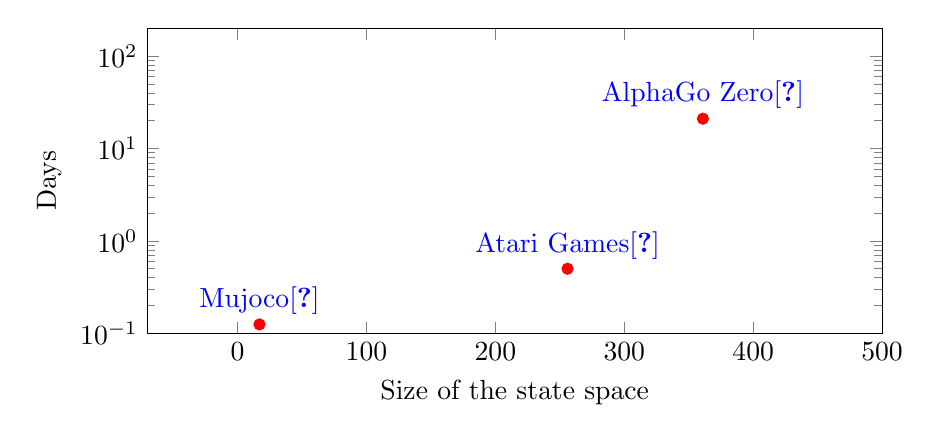
\begin{tikzpicture}
        \begin{axis}[
            ymode=log,
            xmin = -70, xmax = 500,
            ymin = 0.1, ymax = 200,
            xlabel={Size of the state space},
            ylabel={Days},
            % grid = both,
            % xmajorgrids=true,
            % major grid style = {lightgray},
            % minor grid style = {lightgray},
            width = 0.9\linewidth,
            height = 0.45\linewidth,
            nodes near coords=\pgfplotspointmeta,
            point meta=explicit symbolic
        ]
        \addplot[scatter,only marks,mark options={scale=1,fill=red,draw=red},color=blue] table [meta index=2] {
        4 0.01 CartPole
        17 0.125 Mujoco\cite{openai_gym}
        256 0.5 Atari\ Games\cite{openai_gym}
        361 21 AlphaGo\ Zero\cite{alphago_zero}
        };  
        \end{axis}
    \end{tikzpicture}
    \caption{Training time of various environments versus the size of the state space}
    \label{fig:time_vs_state_space}
\end{figure}

\section{Related Work} \label{sec:related_work}
%In this section we put our work into a broader context and provide a summary of other related work, which by no means we claim to be extensive, but rather an overview.
In this section, we situate our work within a broader context and offer a concise summary of other relevant studies.

% DDPMs 
\subsection{Denoising Diffusion Probabilistic Models} Denoising diffusion models are a type of generative deep learning models first formulated by \cite{sohl-dickstein_deep_2015} and further extended to Denoising Diffusion Probabilistic models (DDPMs) by \cite{ho_denoising_2020,nichol_improved_2021}. These models use a Markov Chain to gradually convert one simple and well-known distribution (e.g. a Gaussian distribution) into a usually more complex data distribution the model can sample from. 

% diffusion applications
Diffusion models have been applied to many applications and modalities including image generation \citep{dhariwal_diffusion_2021}, image-to-image translation \citep{saharia_palette_2022}, super-resolution \citep{ho_cascaded_2021, saharia_image_2021}, video \citep{ho_video_2022,harvey_flexible_2022,yang_diffusion_2022}, audio \citep{kong_diffwave_2021,lee_priorgrad_2022}, text-to-image \citep{ramesh_hierarchical_2022, nichol_towards_2022,saharia_photorealistic_2022}, and simultaneous multi-modal generation \citep{ruan_mm-diffusion_2023}.

% generative trilemma
In the generative learning trilemma formulated by \cite{xiao_tackling_2022}, which states that generative models cannot satisfy all three key requirements fast sampling, high quality samples and mode coverage, diffusion models have shown good results in high quality image generation \citep{rampas_novel_2023,ho_cascaded_2021} and mode coverage. While Variational Auto-Encoders (VAEs) \citep{kingma_auto-encoding_2022,razavi_generating_2019} and flow based models \citep{dinh_density_2017,durkan_neural_2019} are strong in covering multi-modal data distributions and can be sampled from very fast, the quality of their samples is usually not as high as of Generative Adversarial Models (GANs) or diffusion models. GANs \citep{goodfellow_generative_2014,brock_large_2019,kirch_vologan_2022} on the other-hand produce high quality images and are sampled quickly but are prone to mode collapse and often do not cover the entire data distribution.

% speed up sampling
DDPMs require many reverse diffusion steps (often several hundreds or even thousands of steps) to sample from, making it difficult train and deploy them even on modern GPUs. Hence it is no surprise that a lot of research focuses on increasing the sample speed of diffusion models by reducing the number of required steps \citep{song_denoising_2022, xiao_tackling_2022, nichol_improved_2021, salimans_progressive_2022,chung_come-closer-diffuse-faster_2022}, perform diffusion in the latent space rather than the full-resolution data distribution \citep{preechakul_diffusion_2022,rombach_high-resolution_2022,sinha_d2c_2021, gu_vector_2022, tang_improved_2023} or formulate the diffusion problem as time-continuous problem to take advantage of accelerated stochastic differential equations (SDE) solvers \citep{song_score-based_2021,song_maximum_2021, song_improved_2020,karras_elucidating_2022}.

% conditional generation
To control the output of the model it must be provided with an additional condition input. The model might be conditioned on another input of the same modality like in colorization \citep{saharia_palette_2022}, inpaintings \citep{batzolis_conditional_2021}, generation from semantic mask \citep{meng_sdedit_2022} or image super-resolution \citep{saharia_image_2021,ho_cascaded_2021}, on an input of different modality like in depth estimation \citep{duan_diffusiondepth_2023} or segmentation \citep{baranchuk_label-efficient_2022}, on class labels \citep{dhariwal_diffusion_2021} or on text prompts \citep{ramesh_hierarchical_2022, nichol_towards_2022,saharia_photorealistic_2022}; to name a few.

Depending on the representation of the condition input, it might be concatenated with the noise input \citep{batzolis_conditional_2021}, fed to multiple layers within the network like adaptive instance normalization \citep{karras_style-based_2019} or via an independent network branch \citep{zhang_adding_2023}. Beside the architectural choice one must also decide how strong the condition should be. One could only apply it for certain time steps in the reverse diffusion process, only apply it during inference on an unconditionally trained model \citep{choi_ilvr_2021} or using guidance, which applies a weighted sum of a conditional and unconditional generation and hence trades-off sample diversity with sample quality. Among others, guidance can be performed with an additionally trained classifier \citep{nichol_improved_2021}, by training the diffusion model conditionally and unconditionally at the same time and sampling using a weighted sum of both \citep{ho_classifier-free_2022} or by using pre-trained CLIP embeddings \citep{nichol_towards_2022,ramesh_hierarchical_2022}.

% Monocular depth estimation
\subsection{Monocular Depth Estimation} Knowledge on the depth of a scene is crucial in a vast number of applications including virtual reality (VR), augmented reality (AR), environment perception, autonomous driving, robotics, state estimation, navigation, mapping and many more. Various surveys \citep{bhoi_monocular_2019,zhao_monocular_2020,ming_deep_2021, masoumian_monocular_2022} summarize the rich and extensive literature on monocular depth estimation; the estimation of the depth based on a single image; an inherently ill-posed and ambiguous problem.

In contrast, conventional geometric-based approaches such as structure from motion and stereo vision matching rely on geometric constraints and multiple viewpoints to reconstruct 3D structures. On the other hand, sensor-based methods leverage dedicated hardware like LiDAR sensors or RGB-D cameras to directly capture depth information. While these methods find practical application, they suffer from significant limitations including high hardware expenses, imprecise and sparse predictions, and limited accessibility for consumer use.

Many different representations can be deployed to obtain depth information: 2D depth maps (dense or sparse), 3D point cloud, 3D pseudo point cloud predicted from other modality (e.g. stereo camera), camera independent disparity maps, light fields, neural radiance fields (NERFs, \cite{mildenhall2021nerf}), 3D meshes, voxels and height maps to name a few.

Numerous deep learning based approaches for monocular depth estimation have been researched in recent years. 
\cite{lu_self-supervised_2022}, \cite{chen_self-supervised_2018} and \cite{zhang_unsupervised_2020} train their models using stereo images while inferring only single view images. The model either learns the correspondence between the two views and can reconstruct the other view or the model incorporates the knowledge of a stereo camera into its weights and hence strengthen its capability to extract meaningful features from a single image. \cite{yue_self-supervised_2022} and \cite{ zhao_joint_2022} apply a multi-task training objective by not only predicting depth but also other related tasks (e.g. normal vector prediction) that help the model to learn a more profound representation and understanding of the scene which also benefits the downstream task of depth estimation.
\cite{watson_temporal_2021} and \cite{bian_unsupervised_2021} use mono camera videos to estimate the depth.

Other deep learning-based approaches focus on multiple sensor modalities to estimate the depth of the scene. \cite{zhang_lidar-guided_2022} use LiDAR point clouds in combination with stereo images, \cite{eldesokey_confidence_2020} use monocular RGB images combined with sparse LiDAR point clouds, \cite{liu_pseudo-lidar_2020} input monocular RGB combined with a depth map and \cite{piao_dynamic_2021} combine a single RGB image with a focal stack.

In this work, we focus on monocular depth estimation using single RGB images as input and generating dense depth maps as output.
We observed that most model architectures are based on GANs, VAEs or similar approaches. We hence further review the usage of diffusion models in the field of depth estimation.

% Depth Diffusion
\subsection{Depth Diffusion}
We observe that very little work has been published on monocular depth estimation using diffusion models. We hypothesize that one of the major reasons is the necessity for fast sampling constraint by real-time applications like autonomous driving. We are certain that the community will find a way to further increase the sampling speed in a future and hence we see great potential in diffusion models for monocular depth estimation.

\cite{saxena_monocular_2023} used a diffusion model to perform monocular depth estimation on indoor and outdoor scenes introducing a preprocessing step to complete incomplete depth data and were even able to resolve depth ambiguity introduced from transparent surfaces.
\cite{duan_diffusiondepth_2023} use a latent diffusion model in combination with a Swin Transformer backbone \citep{liu_swin_2021} to first encode the depth into latent space and then perform the reverse diffusion in the latent space by iteratively applying their light weighted monocular conditioned denoising block. Finally, they apply a fully convolutional decoder on the diffused latent space to obtain the final depth prediction.
\cite{ranftl_towards_2020} propose methods to mix multiple depth datasets for robust training to mitigate the challenges of acquiring dense ground truth data from a variety of scenes. \cite{bhat_zoedepth_2023} proposes a method to combine relative depth and metric depth in a zero-shot manner, by pre-training on a large corpus of relative depth datasets and finetuning on metric depth.

Not as closely related but still applying diffusion models on 3D related data representations, we found \textbf{3D point cloud generation} conditioned on monocular images \citep{zhou_3d_2021}, conditioned on an encoded shape latent \citep{luo_diffusion_2021} and conditioned in CLIP-tokens \citep{nichol_point-e_2022}, \textbf{novel view synthesis} from a single view \citep{rockwell_pixelsynth_2021,watson_novel_2022}, for perpetual view generations for long camera trajectories where depth is predicted as an intermediate representation \citep{liu_infinite_2021} or combining text prompts for 2D generation with Neural Radiance Fields (NeRFs) \citep{poole_dreamfusion_2022}, \textbf{depth estimation} from multiple camera images at different viewpoints \citep{khan_differentiable_2021} and \textbf{depth-aware guidance} methods that guide the image generation process by its intermediate depth representation \citep{kim_dag_2023}.
% \section{The Proposed Method}
\section{Multi-Object Tracking with Memory}
\label{sec:method}

\subsection{Overview}
\label{sec:method:overview}

Given a sequence of video frames $\mathbi{I} = \{I^0, I^1, \cdots, I^T\}$,
the goal of online MOT is to localize a set of $K$ objects while following their trajectories $\mathbfcal{T} = \{\mathcal{T}_0, \mathcal{T}_1, \cdots, \mathcal{T}_K\}$ over time by causal processing.
In this paper, we propose an end-to-end tracking algorithm, called \textit{MeMOT}, which jointly learns the object detection and association.
Different from most existing methods~\cite{bergmann2019tracking} that propagate the states of tracked objects between adjacent frames,
we build a \textit{spatio-temporal memory} that stores long-range states of all tracked objects, together with a \textit{memory encoding-decoding} process that efficiently retrieves useful information for linking objects after a long time span.

Specifically, as shown in Figure~\ref{fig:network}, MeMOT consists of three main components:
1) a frame-level hypothesis generation module $\Theta_H$ that produces region proposals for the current video frame $I^t$,
2) a track-level memory encoding module $\Theta_E$ that aggregates track embeddings,
and 3) a memory decoding module $\Theta_D$ that associates the new detections with tracked objects.
At time step $t$,
$\Theta_H$ generates $N^t_{pro}$ region proposals, represented as proposal embeddings $\mathbi{Q}_{pro}^t \in \mathbb{R}^{N^t_{pro} \times d}$ using a Transformer-based architecture.
The memory encoder $\Theta_E$ adaptively translates the ``history states'' of each track into one compact representation, denoted as track embeddings $\mathbi{Q}_{tck}^t \in \mathbb{R}^{N^t_{tck} \times d}$. 
By querying the encoded image feature with $[\mathbi{Q}_{pro}^t, \mathbi{Q}_{tck}^t]$,
the memory decoder $\Theta_D$ computes the inter-object relations and updates the embeddings as $[\widehat{\mathbi{Q}}_{pro}^t, \widehat{\mathbi{Q}}_{tck}^t]$ accordingly.
Then the locations $[\mathbi{B}_{pro}^t, \mathbi{B}_{tck}^t]$ and confidence scores  $[\mathbi{S}_{pro}^t, \mathbi{S}_{tck}^t]$ of new and tracked objects are predicted based on these output embeddings.
Finally, the locations and states of the previously tracked objects are used to update their trajectory and the memory.
The ``new-born'' objects are initialized in $\mathbfcal{T}$ and their states are added into the memory.

\subsection{Hypothesis Generation}
\label{sec:method:theta_H}

The hypothesis generation network $\Theta_H$ is built with an encoder-decoder architecture based on Transformers~\cite{carion2020end,zhu2020deformable}.
It produces a set of $N^t_{pro}$ region proposals that either initiate ``new-born'' objects for the current video frame or update tracked objects with their latest identity and position information.
The $\Theta_H$ encoder takes a sequentialized feature map $z_0^t \in \mathbb{R}^{C \times HW}$ as inputs, which is extracted by a CNN backbone from the input frame $I^t$.
Each element in $z_0^t$ is supplemented with a unique positional encoding that indicates its spatial location.
The image feature is encoded as $z_1^t \in \mathbb{R}^{d \times HW}$ using a multi-layer Transformer encoder.
The $\Theta_H$ decoder receives the encoded feature $z_1^t$ and empty object queries (represented as learnable embeddings), and produces the final set of proposal embeddings $\mathbi{Q}_{pro}^t \in \mathbb{R}^{N_{pro}^t \times d} $.
The objectness scores and bounding boxes of each proposal can be predicted from $\mathbi{Q}_{pro}^t$.

\begin{figure}
    \centering
    \includegraphics[width=0.5\textwidth]{figures/memory_module.pdf}
    \vspace{-7.5mm}
    \caption{
        \textbf{Illustration of Memory Aggregator}, which consists three attention modules: 1) short-term $f_{short}$ that smoothes out noises in recent frames, 2) long-term $f_{long}$ that extracts supportive features from long-range context, and 3) fusion blocks that aggregate short- and long-term branches. The aggregated embeddings will be used as the track embeddings (blue-white query) and update DMAT (blue-red query) for the next time step.
        % \textbf{Illustration of Memory Aggregator}, which consists three attention modules: 1) a short-term $f_{short}$, 2) a long-term $f_{long}$, and 3) a fusion block. The aggregated embeddings will be used as the track embeddings (blue-white query) and update DMAT (blue-red query) for the next time step.
    }
    \label{fig:ta}
    \vspace{-4.5mm}
\end{figure}

\subsection{Spatio-Temporal Memory}
\label{sec:method:memory}

We store the history states of all $N$ tracked objects in a spatio-temporal memory buffer $\mathbi{X} \in \mathbb{R}^{N \times T \times d}$.
It reserves at most $N_{max}$ objects and a maximum of $T_{max}$ time steps for each object.
The memory is implemented with a first-in-first-out (FIFO) data structure. 
At time step $t$, the memory is represented as the states of $N_{tck}^{t-1}$ active objects in the past $T$ frames, $\mathbi{X}^{t-1-T:t-1}=\{x_k^{t-1-T:t-1}\}_{k=1:N_{tck}^{t-1}}$, where $x_k^{t-1-T:t-1}$ is the states of the $k$-th object and is padded with $\mathbi{0}$ if this object does not appear in the frame $I^t$.
When $T$ is larger than $T_{max}$, the ``oldest'' state $x_k^{t-1-T}$ of each tracklet graduates from the memory.
$N_{max}$ is set to be significantly large (\eg, 300 or 600) to cover the typical number of objects in a video, and a choice of $T_{max}$ is 24.

\subsection{Memory Encoding}
\label{sec:method:theta_E}

As shown in Fig.~\ref{fig:ta}, we encode the memory and extract the track embedding with three attention modules:
1) a short-term block $f_{short}$ for assembling embeddings of neighboring frames to smooth out the noises,
2) a long-term block $f_{long}$ for extracting relevant features in the temporal window covered by the memory,
and 3) a fusion block $f_{fusion}$ for aggregating embeddings from short- and long-term branches.

For each tracklet, the short-term module $f_{short}$ takes as inputs its previous $T_s$ states while the long-term memory module $f_{long}$ utilizes longer history with length of $T_l$ ($T_s \ll T_l$).
$f_{short}$ and $f_{long}$ are implemented with multi-head cross-attention modules, where the history states are key and value inputs.
% We assume that the observations in the current frame are closer to those in the nearby frames and the long-term memory contains more redundant but supportive information.
The input query for $f_{short}$ is the most recent state $\mathbi{X}^{t-1}$, while an dynamically updated embedding, called \textit{Dynamic Memory Aggregation Tokens (DMAT)}, $\mathbi{Q}^{t-1}_{dmat} = \{{q_{dmat}}_k^{t-1}\}_{k=1:N_{tck}}$ is used for $f_{long}$.
When every tracklet is initiated, it is associated with the same DMAT as others; after that, at time step $t > 0$, DMAT is iteratively updated from the previous step. This design will be further validated in Sec.~\ref{sec:exp:ablation}.
The outputs of the short- and long-term branches, denoted as \textit{Aggregated Short-term Token (AST)} $\mathbi{Q}^t_{AST}$ and \textit{Aggregated Long-term Token (ALT)} $\mathbi{Q}^t_{ALT}$, are then fused by $f_{fusion}$.
It outputs the track embedding $\mathbi{Q}_{tck}^t$ and an updated $\mathbi{Q}^{t}_{dmat}$ where the latter is retained for the next timestep. 

\subsection{Memory Decoding}
\label{sec:method:theta_D}

The memory decoder $\Theta_D$ takes the proposal embedding, track embedding, and the image feature as inputs to produce the final tracking results. 
It is realized by using stacked Transformer decoder units, where the concatenated proposal and track embeddings $[\mathbi{Q}^t_{pro}, \mathbi{Q}^t_{tck}]$ are used as queries.
$\Theta_D$ takes the encoded image feature $z_1^t$ from $\Theta_H$ as key and value.

For each entry $q_i^t$ in $\Theta_D$'s outputs $[\widehat{\mathbi{Q}}^t_{pro}, \widehat{\mathbi{Q}}^t_{tck}]$, the decoding process generates three predictions: the bounding box (in the format of offsets \wrt the learned reference points), the \emph{objectness score}, and the \emph{uniqueness score}.
The objectness score $o_{i}^t$ for a query $q_i^t$ ranges from $0$ to $1$, where $o_{i}^t=1$ means the model determines the entry is depicting a visible object.
The uniqueness score $u_i^t$ also ranges from $0$ to $1$. When $u_i^t=1$ the model predicts that the object depicted by $q_i^t$ is unique and should be included in the tracking outputs. Otherwise it needs to be suppressed. We define that $u_i^t=1$ if $q_i^t\in \widehat{\mathbi{Q}}^t_{tck} $. When the model learns to predict $u_i^t$ for each proposal entry, we enforce that a proposal is only considered novel ($u_i^t=1$) when it is not related to any object being tracked. 
We can then define a unified \textbf{confidence score} for both proposal and track entries as the multiplication of objectiveness and uniqueness scores:
% as $s_k^t = o_k^t \cdot u_k^t$:
%
\vspace{-1.0mm}
\begin{equation}
s_k^t = 
    o_k^t \cdot u_k^t.
\label{eq:score}
\end{equation}
\vspace{-1.0mm}
%
The predicted confidence scores of the proposal and track queries are referred to as $\mathbi{S}^t_{tck}$ and $\mathbi{S}^t_{pro}$, respectively. 
For each entry $q_i^t$, the model predicts its bounding box $\mathbf{b}_i^t$, where $\mathbf{b}_i^t \in \mathbb{R}^{4 \times 1}$ includes the object's center coordinates, width, and height. 

The above formulation allows us to solve the object detection and data association problem simultaneously.
In inference, we threshold each entry of $[\widehat{\mathbi{Q}}^t_{pro}, \widehat{\mathbi{Q}}^t_{tck}]$ with the threshold $\epsilon$ and only retain entries with $s_i^t \ge \epsilon$. The resulted entries will automatically bear an track identity or initialize a new track according to whether they come from  $\widehat{\mathbi{Q}}^t_{pro}$ or $\widehat{\mathbi{Q}}^t_{tck}$.
We can then obtain the final tracking results by combining the inherited or newly formed track identities with the corresponding bounding box prediction. There is \emph{no} need for further post processing~\cite{wojke2017simple,bergmann2019tracking,zhang2020fair}. 

To generate the supervision signals for $o_i^t$, $u_i^t$, and $\mathbf{b}_i^t$ on each frame, we first assign the objectiveness score and bounding box to entries in $\widehat{\mathbi{Q}}^t_{tck}$ based on whether the tracked object is present in this frame. 
Then for each entry in $\widehat{\mathbi{Q}}^t_{pro}$, we assign the groundtruth bounding boxes, regardless of new or already tracked, to each entry through bipartite matching~\cite{erhan2014scalable,carion2020end}.
Then we assign the groundtruth uniqueness score to each proposal entry, as shown in Fig.~\ref{fig:asso_solver}, based on whether its matched object has been seen before. 

\begin{figure}
    \centering
    \includegraphics[width=0.5\textwidth]{figures/asso_module.pdf}
    \vspace{-6.0mm}
    \caption{\textbf{Illustration of ground truth assignment} to tracked objects, new objects, suppressed objects, and backgrounds. We show the assigned groundtruth scores for each type of entry.}
    \label{fig:asso_solver}
    \vspace{-4.0mm}
\end{figure}

\subsection{Training MeMOT}
\label{sec:method:training}

We supervise MeMOT with the \textit{tracking loss} computed on the $o_i^t$, $u_i^t$, $\mathbf{b}_i^t$ following the assignment process above as
%
\begin{equation}
%\small
    L_{tck} = \lambda_{cls}(L'_{obj}+L'_{uni})+\lambda_{L_1}L'_{bbox}+\lambda_{iou}L'_{iou},
\end{equation}
%
where $\lambda$s are hyper-parameters for weight scaling, $L_{obj}$ and $L_{uni}$ are focal loss on objectness scores and uniqueness scores, $L_{bbox}$ is L1 loss for bounding box regression, $L_{iou}$ is the generalized IoU loss~\cite{rezatofighi2019generalized}.

Additionally, we apply a detection loss to the proposal embedding similar to Deformable DETR's~\cite{zhu2020deformable} to enhance MeMOT's localization capability.
Specifically, we attach an auxiliary linear decoder to the proposal embedding to output bounding boxes and object classification scores. We then assign the object instances to them as in normal object detection tasks~\cite{zhu2020deformable} and similarly compute the loss as
%
\begin{equation}
%\small
   L_{det} = \lambda_{cls}L_{obj}+\lambda_{L_1}L_{bbox}+\lambda_{iou}L_{iou}.
\end{equation}
%
Note the auxiliary decoder is discarded after training. 

% , which is matched by the Hungarian algorithm, while those for the $\Theta_D$'s are determined by object identities (\ie, each query is responsible for a track).
% Formally, given the prediction results from the $\Theta_H$ decoder and $\Theta_D$ as $\hat{Y}_\tau$ and $\hat{Y'}_\tau$, respectively, their \textit{matched} ground truths are $Y_\tau$ and $Y'_\tau$ (depending on whether the object identity is considered), the losses are formulated as:
% %
% \begin{equation}
% \footnotesize
%     \begin{split}
%     L_{det}(Y_i,\hat{Y}_i) = &\lambda_{cls}L_{obj}+\lambda_{L_1}L_{bbox}+\lambda_{iou}L_{iou}, \\ 
%      L_{tck}(Y'_i,\hat{Y'}_i) = & \lambda_{cls}(L'_{obj}+L'_{uni})+\lambda_{L_1}L'_{bbox}+\lambda_{iou}L'_{iou},
%     \end{split}
% \end{equation}
% %
% where $\lambda$s are hyper-parameters for weight scaling, $L_{obj}$ and $L_{uni}$ are focal loss on objectness scores and uniqueness scores, $L_{bbox}$ is L1 loss for bounding box regression, $L_{iou}$ is the generalized IoU loss~\cite{rezatofighi2019generalized}.

%$L_{cls}$ is the objectness score $\hat{Y}_i$ and confidence score for $\hat{Y'}_i$ (defined in Eq.~\ref{eq:score}).

Following MOTR~\cite{zeng2021motr}, we compute the tracking loss in a clip by the sum of all individual track queries' losses normalized by the total number of object instances.
For a clip with $T$ frames, the overall loss $L_{clip}$ is a combination of the tracking loss and auxiliary detection loss as:
%
\begin{equation}
    \footnotesize
    \begin{split}
    L_{clip} &= \lambda_{tck}L_{clip-tck}+\lambda_{det}L_{clip-det} \\
    &=\frac{\lambda_{tck}}{\sum_{t=0}^{T} N_t}\sum_{t=0}^T\sum_{i=0}^{|\mathbi{Q}^t_{tc}, \mathbi{Q}^t_{pro}|}{L_{tck}^{(i, t)}}+\frac{\lambda_{det}}{T}\sum^T_{t=0}\frac{1}{N_t}\sum_{j=0}^{|\mathbi{Q}^t_{pro}|}L_{det}^{(j, t)},
    \end{split}
    \label{eq:cliploss}
\end{equation}
%
where $\lambda_{tck} \in \mathbb{R}$ and $\lambda_{det} \in \mathbb{R}$ are the loss weights for balancing the tracking loss and the auxiliary detection loss, respectively. 
Here $N_t$ denotes the total number of visible objects in the frame at time $t$.

%(\ie, new objects plus tracked objects) of bounding boxes in frame $t$.
\section{Experiments}
Our experiments aim to answer the following questions:
\begin{enumerate}
    \item How does our proposed Prioritized Replay Buffer compare against existing baseline approaches? (See Section~\ref{sec:comp_baselin})
    \item Does the performance of our proposed Prioritized Replay Buffer follow the theoretical analysis in Section~\ref{sec:sum_tree} in terms of the fanout size $K$? (See Section~\ref{sec:perf_prioritized})
    \item How does our proposed locking mechanisms for the prioritized replay buffer reduce the synchronization overhead compared with using a global lock? (See Section~\ref{sec:perf_prioritized})
    \item What is the performance improvement when plugging in our prioritized replay buffer implementation into existing RL frameworks? (See Section~\ref{sec:comp_existing})
\end{enumerate}

\subsection{Experimental Setup}
We conduct our experiments on 56-core Intel(R) Xeon(R) Gold 5120 CPUs with 128GB DDR4 memory and a Nvidia TITAN Xp GPU with 12GB GDDR6 memory as the accelerator. We implement the synchronization mechanism using pthreads \cite{pthread} and the training of neural networks using LibTorch \cite{pytorch}. We test our framework on reinforcement learning algorithms including DQN \cite{dqn} and DDPG \cite{ddpg}. DQN targets at discrete action space while DDPG and SAC targets at continuous action space. We use \textit{LunarLander-v2} \cite{openai_gym} environment to test the algorithms. In all our experiments, the desired ratio between the throughput of the data collection and the data learning (update\_interval) is set to 1.

\subsection{Baseline Approach}
In this work, we use RLlib \cite{ray_rllib} as our baseline. RLlib is an open source implementation of parallel and distributed framework for training reinforcement learning agents written in Python \cite{python}. For fair comparison, we use the same amount of cores when running the experiments. We also compare with the Prioritized Replay Buffer implementation in open source RL framework tianshou \cite{tianshou}.

\subsection{Comparison with Baseline Approaches}\label{sec:comp_baselin}
\begin{figure}
    \centering
    \includegraphics[width=\linewidth]{sum_tree_comp.pdf}
    \caption{Comparison with the baseline approach}
    \label{fig:baseline_comp}
\end{figure}

We show the latency of insertion and sampling of the Replay Buffer with various sizes in Figure~\ref{fig:baseline_comp}. We compare our $K$-ary sum tree based implementation with RLlib \cite{ray_rllib} and tianshou \cite{tianshou}. Overall, our approach reduces the total latency by around 4x compared with tianshou \cite{tianshou} and around 100x compared with RLlib \cite{ray_rllib}. Note that the latency of the Prioritized Replay Buffer operations in  RLlib increases in linear while the latency of our implementation increases in sub-linear. This suggests our $K$-ary based Prioritized Replay Buffer has better scalability compared with \cite{ray_rllib}.

\subsection{Performance of the Prioritized Replay Buffer}\label{sec:perf_prioritized}
\begin{figure}
    \centering
    \includegraphics[width=\linewidth]{sum_tree_ops.pdf}
    \caption{Latency of various Prioritized Replay Buffer operations with various fannout $K$}
    \label{fig:k_ary_sum_tree}
\end{figure}
\subsubsection{Effect of fanout $K$}
In order to answer question 2, we show the latency of insertion and sampling of various $K$ in Figure~\ref{fig:k_ary_sum_tree}. We also vary the capacity of the Replay Buffer to demonstrate the scalability. First, we observe that the latency of insertion decreases when $K$ increases. This matches our theoretical performance analysis because the latency is proportion to the height of the tree. The height of the tree decreases when $K$ increases. Second, we observe that the latency of sampling first decreases to a local minimum and then increases as $K$ increases. This also matches with our theoretical analysis because as $K$ increases, the latency increase of search over each level starts to dominate the latency decrease with fewer number of levels. In order to choose the optimal $K$, we simply perform profiling of insertion and sampling to obtain the total latency. In our experimental machine, $K=16$ yields the best result.

\subsubsection{Effect of synchronization optimization}

\begin{figure}
    \centering
    \includegraphics[width=\linewidth]{sum_tree_sync.pdf}
    \caption{Execution time of the Prioritized Replay Buffer with various synchronization methods}
    \label{fig:scalability}
\end{figure}
In order to answer question 3, we show the execution time of 5000 iterations versus the number of CPU cores using a global lock, no lock and our proposed synchronization optimization in Section~\ref{sec:thread_safe_prb}. Although the results of computations without using lock are wrong, it provides an upper bound on the performance. We observe that our proposed thread-level synchronization enables 1.01x$\sim$5x increase of the execution time compared with the minimum achievable execution time; and achieves 2x$\sim$5x improvement against using a global lock. Moreover, our design scales well in the number of CPU cores.


% In order to answer question 2 and 3, we compare the throughput speedup of our proposed prioritized replay buffer using $K$-ary sum tree with the implementation using a binary sum tree with a single global lock. To do so, we spawn 4 threads, each thread runs sampling and priority update on the shared replay buffer using random data 1000 times. The throughput speedup is shown in Figure~\ref{fig:k_ary_sum_tree}. First, we notice that all the throughput speedup is above 4. This is because using a global lock on the replay buffer limits the maximum number of running thread to 1. On the contrary, our proposed locking mechanism provides linear scalability.

% To answer question 3, we observe that there exists a local maximum of the throughput speedup when increasing the fanout size of the sum tree $K$. For example, we choose $K=256$ when the size of the replay buffer is $1000$, $K=128$ when the size of the replay buffer is $10000$ and $K=64$ when the size of the replay buffer is $100000$. It is also worth noticing that the optimal $K$ decreases as the size of the replay buffer increases. This is because as the size of the replay buffer increases, the linear search of the child nodes in one level dominates.

% \subsection{Scalability Analysis}\label{sec:scale_analysis}
% We compare our proposed parallel framework with various CPU cores against the sequential version on various RL algorithms. We show the scalability of our propose framework in Figure~\ref{fig:scalability}. We notice that the performance scales in linear when the number of CPU cores is below 4. The scalability saturates when the number of cores is above 6. The reason is that the bottleneck of the system becomes the GPU, which performs gradient computations and aggregations.





\subsection{Performance improvement of existing frameworks using our proposed replay buffer}\label{sec:comp_existing}
In order to show the superiority of our proposed Prioritized Replay Buffer, we write a Python binding of the C++ implementation and plug it into existing open source RL framework RLlib \cite{ray_rllib}. We show the latency of each training step of two RL algorithms in Figure~\ref{fig:library_perf}. 
Overall, we achieve 1.19x$\sim$ 1.75x performance improvement using various CPU cores.
The speedup decreases as the number of CPU cores increases. This is because the proportion of the replay buffer operations time decreases for each core and the bottleneck shifts to training the neural networks.

\begin{figure}
    \centering
    \includegraphics[width=\linewidth]{state_of_the_art.pdf}
    \caption{Overall speedup by plugging our prioritized replay buffer implementation into existing open source reinforcement learning libraries.}
    \label{fig:library_perf}
\end{figure}

% \subsection{The agent performance of out-of-order execution}

\subsection{Design Space Exploration}

\begin{figure}
    \centering
    \includegraphics[width=\linewidth]{design_space.pdf}
    \caption{Illustration of design space exploration}
    \label{fig:design_space}
\end{figure}

As discussed in Section~\ref{sec:design_space_exp}, the objective is to allocate the number of cores for actors and learners, respectively such that the desired throughput ratio of the data collection and the data consumption is met. Our framework will first profile the throughput curve of actors and learners. We show an example in Figure~\ref{fig:design_space}, where the desired throughput ratio is 1. Then, we perform exhaustive search to find the solution $x_a$ and $x_b$ of Equation~\ref{eq:design_space}. The time complexity of the exhaustive search is $O(M^2)$, where $M$ is the total number of cores in the processor.

\subsection{Impact of the Data Layout}
The total size of the sum tree used in a typical replay buffer of size 1 million is less 10 KB. This makes the whole sum tree fit into the L2 cache of the modern CPUs. Thus, we only observe around $1\%$ benefit of our proposed cache aligned data layout. However, as the increase of the replay buffer size on larger problems, the superiority of our proposed data layout will appear.

\section{Conclusion}
\label{sec:conclusion}
LLMs are swiftly gaining popularity across diverse domains. In our study, we spotlight techniques designed to enhance the LLM's ability to accurately identify the appropriate API for a specific task—a significant but often overlooked aspect in the advancement of this technology. Since APIs function as a universal language enabling diverse systems to communicate effectively, their correct usage can boost the ability of LLMs to interact with tools in the wider world.
In this paper, we propose \oursmethod{}, a new novel pipeline for finetuning LLMs to call APIs. The finetuned model's performance surpasses prompting the state-of-the-art LLM (GPT-4) in three massive datasets we collected. \gorilla{} generates reliable API calls to ML models without hallucination, demonstrates an impressive capability to adapt to test-time API usage changes, and can satisfy constraints while picking APIs. 

\section{Comparison of Reported and Reproduced Performance}
Detailed comparison scores of reported and reproduced performance are shown in \Cref{tab:performance_comparison}.

\begin{table}[ht!]
    \centering
    \small
    \begin{tabular}{lcc}
        \toprule
        {\textbf{Method}} & Reported & Reproduced \\
        \midrule
         GPT 3.5 Turbo 0613 + CoT & 41.5 & 35.2 \textcolor{red}{{\tiny 
         -32.5\%}} \\
         GPT 3.5 Turbo 0613 + DFS & 54.5 & 53.2 \textcolor{red}{{\tiny 
         -2.4\%}}\\
         ToolLLaMA v2 + CoT & 25.0 & 15.0 \textcolor{red}{{\tiny 
         -40\%}} \\
         ToolLLaMA v2 + DFS & 57.0 & 34.0 \textcolor{red}{{\tiny 
         -40.4\%}}\\
         \bottomrule
    \end{tabular}
    \caption{Comparison of performance (Pass Rate) reported in the paper and reproduced by us of ChatGPT and ToolLLaMA v2 on the I1-Instruction group of ToolBench. }
    \label{tab:performance_comparison}
\end{table}

\section{Statistics of API change information}
Detailed statistics of API change categories and information are shown in \Cref{tab:api_change} and \Cref{tab:api_not_available}.

\begin{table}[h!]
    \centering
    \small
    \begin{tabular}{lcc}
     \toprule
    \textbf{Status Type} & \textbf{Number} & \textbf{Percentage} (\%) \\
    \midrule
    % Not Available & 7504 & 45.6 \\
    Not Available & 8095 & 49.2 \\
    % \quad-- Not Connectable & 2426 & 14.7 \\
    % \quad-- Not Found & 583 & 3.5 \\
    % \quad-- Parameter Issues & 591 & 3.6 \\
    % \quad-- Other issues & 4495 & 27.3 \\
    Not Authorised & 1058 & 6.4 \\
    % Parameter Change & 591 & 3.6 \\
    Success & 7311 & 44.4 \\
     \bottomrule
    \end{tabular}
    \caption{APIs changed in ToolBench.}
    \label{tab:api_change}
\end{table}



\begin{table}[h!]
    \centering
    \small
    \begin{tabular}{lcc}
     \toprule
    \textbf{Status Type} & \textbf{Number} & \textbf{Percentage} (\%) \\
    \midrule
    Not Connectable & 2426 & 30.0 \\
    Not Found & 583 & 7.2 \\
    Parameter Change & 591 & 7.3 \\
    Parsing Error & 4247 & 52.6 \\
    Other & 248 & 3.1 \\
    \midrule
    Total & 8095 & 100 \\
     \bottomrule
    \end{tabular}
    \caption{Categories of Not Availability in ToolBench.}
    \label{tab:api_not_available}
\end{table}


% \section{Stability Test Scores with Virtual API Systems}
% Detailed stability test scores are shown in \Cref{tab:real_api_stability_test}.

% \begin{table}[]
%     \centering
%     \small
%     \resizebox{\linewidth}{!}{
%     \begin{tabular}{lcccc}
%         \toprule
%         \multirow{2}{*}{\textbf{Method}} & \multicolumn{4}{c}{\textbf{Percentage of Failing Tools}}\\
%         % \cmidrule{2-5}
%           & 0\% & 10\% & 20\% & 50\% \\
%         \midrule
%          GPT 3.5 Turbo 0613 + CoT & 20.3{\tiny $\pm{0.8}$}  & 17.9{\tiny $\pm{1.2}$} & 16.3{\tiny $\pm{0.6}$} & 12.8{\tiny $\pm{1.7}$} \\
%          GPT 3.5 Turbo 0613 + DFS & 26.6{\tiny $\pm{0.3}$} & 23.9{\tiny $\pm{1.1}$} & 23.2{\tiny $\pm{1.0}$} & 16.3{\tiny $\pm{1.2}$}\\
%          GPT 4 0613 + CoT & 21.4{\tiny $\pm{0.5}$}  & 19.6{\tiny $\pm{0.9}$} & 15.5{\tiny $\pm{0.3}$} & 11.8{\tiny $\pm{0.8}$} \\
%          GPT 4 0613 + DFS &  24.2{\tiny $\pm{1.8}$}  & 24.0{\tiny $\pm{0.8}$} & 21.2{\tiny $\pm{1.8}$} & 16.9{\tiny $\pm{0.4}$}\\
%          \bottomrule
%     \end{tabular}
%     }
%     \caption{SoPR change when manually make APIs down on the I1 Instruction group.}
%     \label{tab:real_api_stability_test}
% \end{table}
\section{Stability Test Scores with Virtual API Systems}
\label{app:detailed_stability_test_virtual}
Detailed scores of stability tests of various models are shown in \Cref{tab:simulated_api_stability_test}. Note that in addition to GPT 3.5 Turbo 0613 and GPT 4 0613, we report the performance of newer versions, namely GPT 3.5 Turbo 1106 and GPT 4 Turbo Preview.
\begin{table}[]
    \centering
    \small
    \resizebox{\linewidth}{!}{
    \begin{tabular}{ccccc}
        \toprule
        \multirow{2}{*}{\textbf{Method}} & \multicolumn{4}{c}{\textbf{Real API Failure Rate}}\\
        \cmidrule{2-5}
          & 0\% & 10\% & 20\% & 50\% \\
        \midrule
         GPT 3.5 Turbo 0613 + CoT & 49.1{\tiny $\pm{1.0}$}  & 48.7{\tiny $\pm{0.9}$} & 51.2{\tiny $\pm{1.3}$} & 49.0{\tiny $\pm{0.7}$} \\
         GPT 3.5 Turbo 0613 + DFS & 68.1{\tiny $\pm{1.4}$}  & 70.9{\tiny $\pm{1.3}$} & 67.5{\tiny $\pm{1.8}$} & 67.3{\tiny $\pm{1.3}$}\\
         GPT 4 0613 + CoT & 55.4{\tiny $\pm{0.6}$}  & 55.5{\tiny $\pm{1.0}$} & 58.0{\tiny $\pm{0.5}$} & 55.2{\tiny $\pm{0.6}$} \\
         GPT 4 0613 + DFS & 69.7{\tiny $\pm{1.4}$}  & 71.4{\tiny $\pm{1.4}$} & 71.2{\tiny $\pm{0.9}$} & 69.9{\tiny $\pm{0.9}$}\\
         \midrule
         GPT 3.5 Turbo 1106 + CoT & 52.1{\tiny $\pm{0.7}$}  & 52.4{\tiny $\pm{0.8}$} & 53.9{\tiny $\pm{0.6}$} & 50.2{\tiny $\pm{0.6}$} \\
         GPT 3.5 Turbo 1106 + DFS & 69.9{\tiny $\pm{0.7}$}  & 71.7{\tiny $\pm{0.7}$} & 69.4{\tiny $\pm{0.8}$} & 71.6{\tiny $\pm{0.9}$}\\
         GPT 4 Turbo preview + CoT & 60.8{\tiny $\pm{0.7}$}  & 62.8{\tiny $\pm{0.5}$} & 64.2{\tiny $\pm{0.7}$} & 62.4{\tiny $\pm{0.5}$} \\
         GPT 4 Turbo preview + DFS& 73.2{\tiny $\pm{1.1}$}  & 76.7{\tiny $\pm{1.0}$} & 76.0{\tiny $\pm{0.8}$} & 74.2{\tiny $\pm{1.3}$}\\     
         \bottomrule
    \end{tabular}
    }
    \caption{Performance change when manually make APIs down with our virtual online API system. The results are averaged over all six groups. Solving rates are reported. We run each experiment one time and evaluate three times and take the average score.}
    \label{tab:simulated_api_stability_test}
\end{table}




\section{Call Error Identification and Cache Filtering Rule}\label{app:filter_rule}
We identify call errors and filter out invalid call to RapidAPI based on keyword occurences. In detail, we identify the following error:
\begin{itemize}
    \item Not Connected Error: when error information contains \texttt{HTTP} or the response infomation contains \texttt{HTTP error, connection, rate limit, time(d) out};
    \item Not Found Error: when the error information or response contains \texttt{not found, not available, API doesn't exists, Service Not Found, internal error} or 404 error message;
    \item Parameter Change: when the error information or response contains \texttt{parameter, parse, is not defined};
    \item Parsing Error: when the error information starts with \texttt{Function executing from};
    \item Not Authorised: when the error information or response contains \texttt{authoriz(s), unauthoriz(s), blocked user, unsubscribe, credential, disabled for your subscription, ACCESS\_DENIED} or 401, 403 error message;
    \item Other Errors: messages with non-empty error messages;
    \item Success: Other calls.
\end{itemize}
We consider all types of errors when identifying errors. However, when filtering the cache, we do not conside the``Other Errors''.

\begin{table*}[ht!]
    % \small
    \centering
    % \resizebox{\columnwidth}{!}{
    \begin{tabular}{p{0.1\textwidth}p{0.8\textwidth}}
    \toprule
    \rowcolor[gray]{0.95} 
    \multicolumn{2}{c}{\textbf{API Simulation Prompt}} \\
    \midrule
    System & \makecell[{{p{.8\textwidth}}}]{
    Imagine you are an API Server operating within a specialized tool, which contains a collection of distinct APIs. Your role is to deeply understand the function of each API based on their descriptions in the API documentation. As you receive specific inputs for individual API calls within this tool, analyze these inputs to determine their intended purpose. Your task is to craft a JSON formatted response that aligns with the expected output of the API, guided by the provided examples. \\
    Your responses must adhere to a specific JSON structure, which is as follows: \\
    \texttt{\{
        ``error'': ``'',
        ``response'': ``Your\_Response''
    \}}\\
The error field should remain empty, indicating no errors in processing. The response field should contain the content you formulate based on the API's functionality and the input provided. Ensure that your responses are meaningful, directly addressing the API's intended functionality. If the provided examples are mostly error messages or lack substantial content, use your judgment to create relevant and accurate responses. The key is to maintain the JSON format's integrity while ensuring that your response is an accurate reflection of the API's intended output within the tool.\\
Please note that your answer should not contain anything other than a json format object, which should be parsable directly to json. \\
Note that: \\
- your response should be around 100 to 200 words, containing rich information given the api input parameters. Keep Your answer short and simple.\\
- your response must be effective and have practical content.\\
- if the api response example if null or ineffective, ignore the example and give your independent response. \\
    } \\
    \hline
    User & \makecell[{{p{.85\linewidth}}}]{
    API Documentation:\\
    \texttt{Documentation JSON file}\\
    API Examples: \\
    \texttt{Example input 1: Example response 1}\\
    \texttt{Example input 2: Example response 2}\\
    \texttt{Example input 3: Example response 3}\\
    API input:\\
    \texttt{Argument JSON string, e.g:} \\
    \texttt{\{``category'':``Logistics'',}\texttt{``tool\_name'': ``SQUAKE'',}\\
    \texttt{``api\_name'': ``Checkhealth'',``tool\_input'': ``\{\}'',}\\
    \texttt{``strip'': ``filter''\}}
    } \\
    \bottomrule
    \end{tabular}
    \caption{Prompt used to simulate APIs.}
    \label{tab:prompt_simulate_api}
\end{table*}

\begin{table*}[ht!]
    % \small
    \centering
    % \resizebox{\columnwidth}{!}{
    \begin{tabular}{l}
    \toprule
    \rowcolor[gray]{0.95} 
    \textbf{Solvable Task Filtration Prompt} \\
    \midrule
    \makecell[l{p{\textwidth}}]{
    Please check whether the given task solvable with following rules:\\
    1. If the \texttt{query} provide invalid information (e.g. invalid email address or phone number), return \texttt{Unsolvable}\\
    2. If the \texttt{query} needs more information to solve (e.g. the target restaurant name in a navigation task), return \texttt{Unsolvable} \\
    3. If the current \texttt{available\_tools} are enough to solve the query, return \texttt{Solvable} \\
    4. Return only \texttt{Solvable} or \texttt{Unsolvable} \\
    \\
    Task:\{\texttt{task}\}
    \\
    Now please give your answer (only \texttt{Solvable} or \texttt{Unsolvable}):
}
    \\
    \bottomrule
    \end{tabular}
    \caption{Prompt used to filter solvable tasks.}
    \label{tab:task_solvability}
\end{table*}

\section{Configurations of API Diversity Analysis }\label{app:diversity_conf}
The configurations of diversity analysis are as follows:
\begin{itemize}
    \item Embedding model: \texttt{all-mpnet-base-v2};
    \item UMAP metric (distance metric): correlation;
    \item Num of neighbours: 15;
    \item Min distance: 0.5.
\end{itemize}


\section{Prompts of API simulation}
\label{app:prompt_simulation}


The prompt used to simulate API behaviours is shown in \Cref{tab:prompt_simulate_api}.


\section{Prompt to Filter Solvable Task}
\label{app:prompt_task_solvability}
The prompt used to filter solvable tasks is shown in \Cref{tab:task_solvability}.




\section{Prompt Used to Make API Calls}\label{app:prompt_make_call}
The prompt used to construct API calls to scan availables is shown in \Cref{tab:prompt_api_call}.

\begin{table*}[t!]
    % \small
    \centering
    % \resizebox{\columnwidth}{!}{
    \begin{tabular}{p{0.1\textwidth}p{0.8\textwidth}}
    \toprule
    \rowcolor[gray]{0.95} 
    \multicolumn{2}{c}{\textbf{API Call Writing Prompt}} \\
    \midrule
    System & \makecell[{{p{.8\textwidth}}}]{
Imagine you are an API requester, Your role is to deeply understand the function of each API based on their descriptions in the API documentation.  Your task is to craft a JSON formatted input that aligns with the expected input of the API, guided by the provided examples.\\
Your responses must adhere to a specific JSON structure, which is as follows:\\
Please note that your answer should not contain anything other than a json format object, which should be parsable directly to json. \\
Note that:\\
- your response should be around 100 to 500 words, containing rich information given the api input parameters.\\
- your response must be effective and have practical content.\\
- if the api response example if null or ineffective, ignore the example and give your independent response.\\
    } \\
    \hline
    User & \makecell[{{p{.85\linewidth}}}]{
    API Documentation:\\
    \texttt{Documentation JSON file}\\
    API Examples (if available): \\
    \texttt{Example input 1: Example response 1}\\
    \texttt{Example input 2: Example response 2}\\
    \texttt{Example input 3: Example response 3}\\
    one more API Input example:\\
    } \\
    \bottomrule
    \end{tabular}
    \caption{Prompt used to write API calls.}
    \label{tab:prompt_api_call}
\end{table*}







%%%%%%%%% REFERENCES
{\small
\bibliographystyle{ieee_fullname}
\bibliography{egbib}
}

\end{document}
